\documentclass[a4paper,11pt]{kth-mag}
\usepackage[T1]{fontenc}
\usepackage{textcomp}
\usepackage{lmodern}
\usepackage[latin1]{inputenc}
\usepackage[swedish,english]{babel}
\usepackage{modifications}

\usepackage{graphicx}
\usepackage{amsmath}

% Put title here
\title{Weakly Supervised Object Detection: (Working title)}

\subtitle{Duis autem vel eum iruire dolor in hendrerit in
          vulputate velit esse molestie consequat, vel illum
          dolore eu feugiat null}
\foreigntitle{Lorem ipsum dolor sit amet, sed diam nonummy nibh eui
              mod tincidunt ut laoreet dol}
              
\author{Muhammad Iqbal Tawakal}

\date{2015}
\blurb{Master's Thesis at NADA\\Supervisor: Tjoho\\Examiner: Tjohej}
\trita{TRITA xxx yyyy-nn}

\begin{document}
\frontmatter
\pagestyle{empty}
\removepagenumbers
\maketitle
\selectlanguage{english}

\begin{abstract}
  This is a skeleton for KTH theses. More documentation
  regardings the KTH thesis class file can be found in
  the package documentation.
  
  Weakly supervised object detection is...
\end{abstract}

\clearpage
\begin{foreignabstract}{swedish}
  Denna fil ger ett avhandlingsskelett.
  Mer information om \LaTeX-mallen finns i
  dokumentationen till paketet.

\end{foreignabstract}
\clearpage
\tableofcontents*
\mainmatter
\pagestyle{newchap}


\chapter{Introduction}
\label{chap:intro}

% Computer vision history
Computer vision is a field that focused on the process of acquiring, analyzing, and ultimately extracting knowledge and getting comprehensive understanding of the input image. The input image can take many forms such as still image (black and white or colored image), video sequences, multiple input from multiple cameras, and also input from other related sensor. This field has strong ties with other field such as artificial intelligence, machine learning, and robotic.

There are wide range of real world applications for computer vision, starting from simple inspection system in industry and manufacturing process to the creation of robot with artificial intelligence that can interact with  the world around them. Other application include system for navigation (for example autonomous mobile robot and vehicle) and military (security surveillance and missile guidance system).

Those applications can usually be broken down into several small scale vision tasks. Two of the most typical tasks in computer vision are object recognition and object detection. Object recognition tries to predict and identify what class of object is contained inside an image. In detection case, not only the class of the object, the position itself must also be located, usually by marking a tight bounding box closely surrounding the object. Both are hard, challenging problems that are still being actively researched today.

% Reason for difficulty
There are many factors that can be attributed as to why the object recognition and its kind are hard. One reason is simply because the natural representation of image as 2D matrix of pixels value hold little to no direct information that can be used to distinguish different object. Figure \ref{fig:car} illustrate this example. 

This is worsened by the high dimensionality of the data. A standard high definition colored image with the size of 1280x720 can contains up to 2764800 dimensions. Meanwhile the amount of training data rarely exceed or even match this number. This curse of dimensionality can make the training phase to become slow and hard.

\begin{figure}[h]
\centering
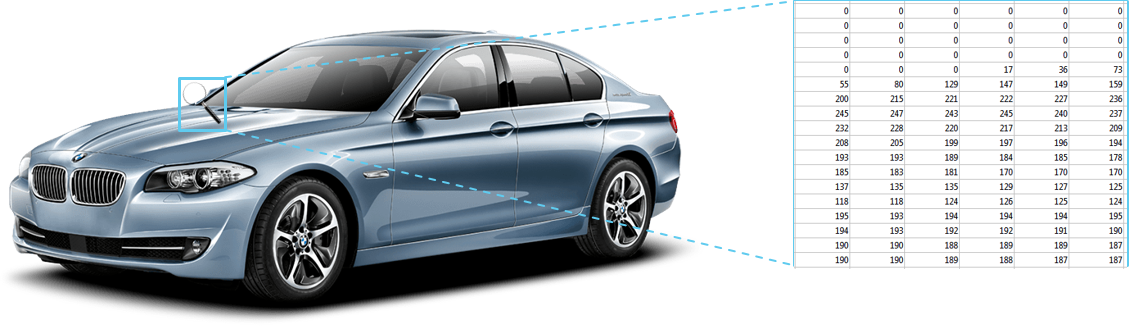
\includegraphics[scale=0.4]{image/car.png}
\label{fig:car}
\caption{The image as 2D matrix of pixels.}
\end{figure}

Furthermore, there are many variations which makes same identical object to have very different appearances in the image. This can be due to viewing changes (translation, rotation, or scale change), change of illumination, occlusion, and clutter. There are also intrinsic difference of object from the same class. Figure \ref{fig:objects} illustrates this example.

\begin{figure}[h]
\centering
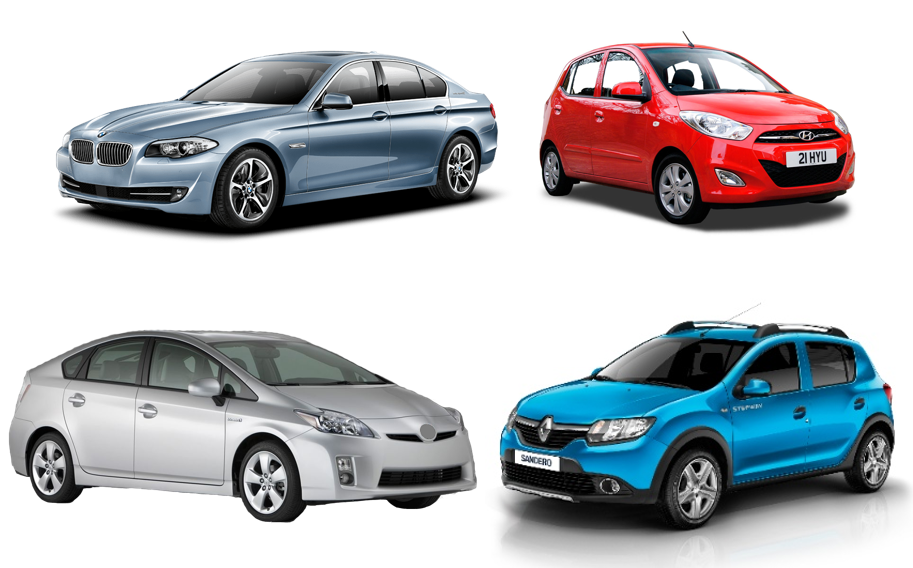
\includegraphics[scale=0.4]{image/cars.png}
\label{fig:cars}
\caption{Object with different appearances, be it color or shape, from the same class.}
\end{figure}

% The importance of features
All this boils down to finding the best representation or features of the said object. An ideal representation would be highly discriminative of different class of object but captures the intrinsic similarity between object from the same class. It also has to be invariant to the object transformation (translation, rotation, and scale invariant), usually have lower number of dimension, and also fast and easy to compute.

Unfortunately, these kind of ideal features do not exist in reality. In practice, we compromise by striking a balance of using adequate number of training data and using a stronger learning algorithm to compensate for the not-so-ideal features. Figure \ref{fig:feature} shows illustration of the ideal features and the not-so-ideal features.

\begin{figure}[h]
\centering
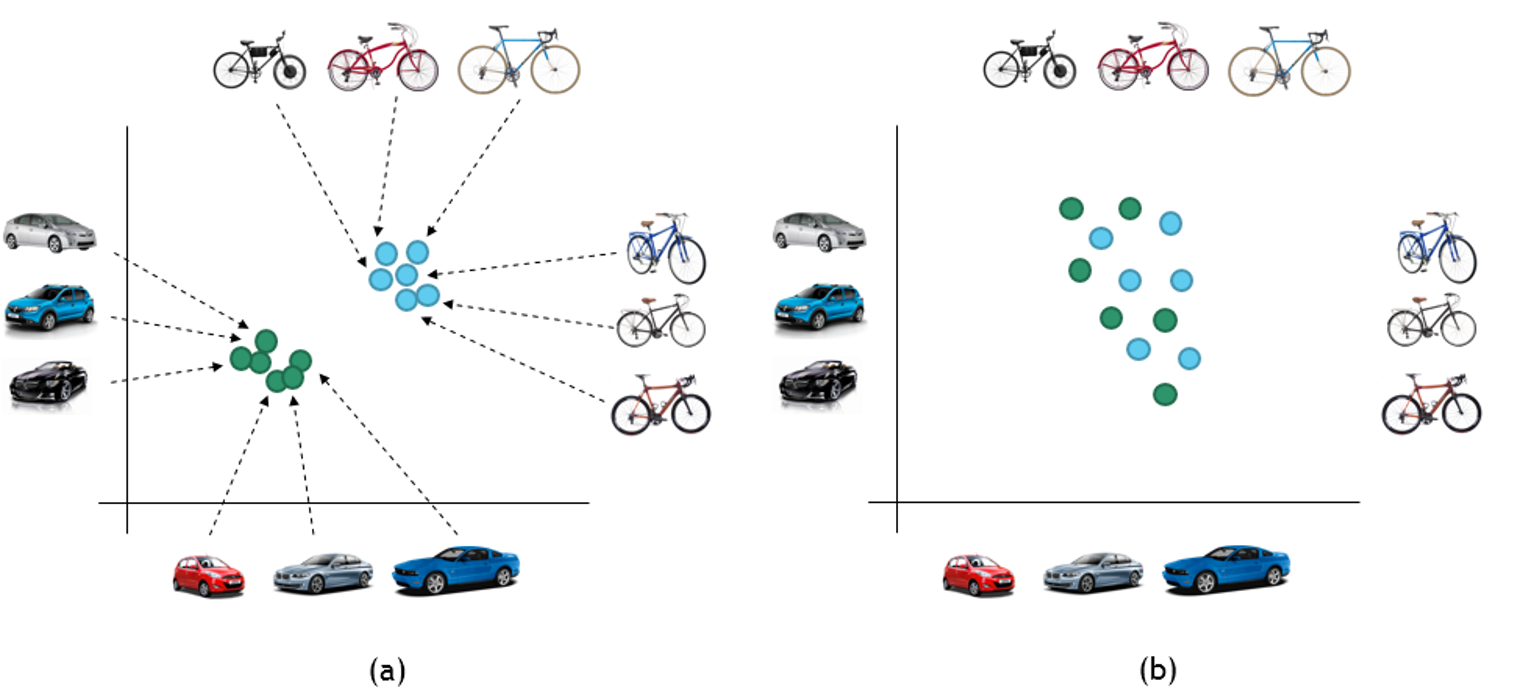
\includegraphics[scale=0.4]{image/ideal_feature.png}
\label{fig:feature}
\caption{Illustration of ideal and not-so-ideal features. (a) Ideal feature should have better separability from instance from different class and closely located with object form the same class. (b) Not-so-ideal features plot is jumbled all over the place and have low separability. This, however, can be compensated by using stronger classification algorithm.}
\end{figure}

% Handcrafted features
Many studies have proposed a wide array of feature extraction techniques. Until very recently, Scale-Invariant Feature Transform (SIFT) by Lowe \cite{lowe2004sift} and Histogram of Oriented Gradients (HOG) by Dalal and Triggs \cite{dalal2005hog} are the leading technique for feature extraction and produced decent performance on benchmark dataset. Both are similar in the sense that both first compute the gradient in the image and then count the gradient based on their direction into a histogram.

\begin{figure}[h]
\centering
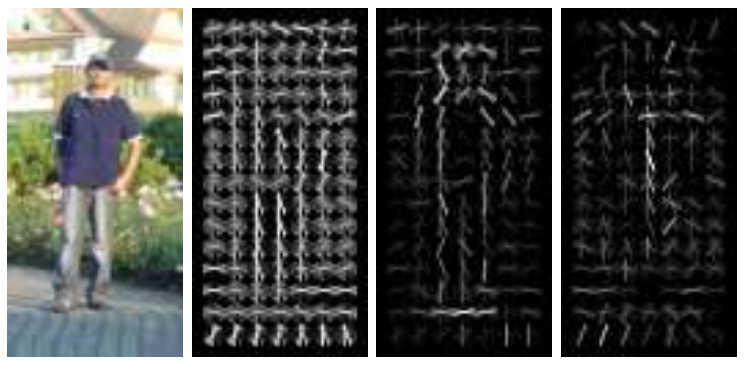
\includegraphics[scale=0.4]{image/hog.png}
\label{fig:hog}
\caption{Illustration of HOG features applied on image of a person.}
\end{figure}

Some study extends these features into mid-level representation by clustering nearby features (using k-means clustering for example). The number of features that fall into a specific cluster is then aggregated into some bag of visual word. However, this kind of hand-crafted features still cannot reach the level of human performance.

The trend shifts, there comes the initiative to learn the features directly from data. This is partly motivated due to the abundance of image data, mostly coming from the internet. There are two different approaches for this, the unsupervised learning and supervised learning.

Unsupervised feature learning works with image without label. It tries to learn generic features of object, regardless of their class. It is more advantageous because most of the data comes unlabeled and the extra effort to annotate the image with labels can be expensive and time-consuming.

One technique that implement this idea is Sparse Autoencoder. In its simplest form, it is a variant of neural network with the number of hidden neuron fewer than the dimension of the input. It then forces the network to learn compressed, low-dimensional representation of the image. Figure \ref{fig:autoencoder} illustrates some example features learned from this network.

\begin{figure}[h]
\centering
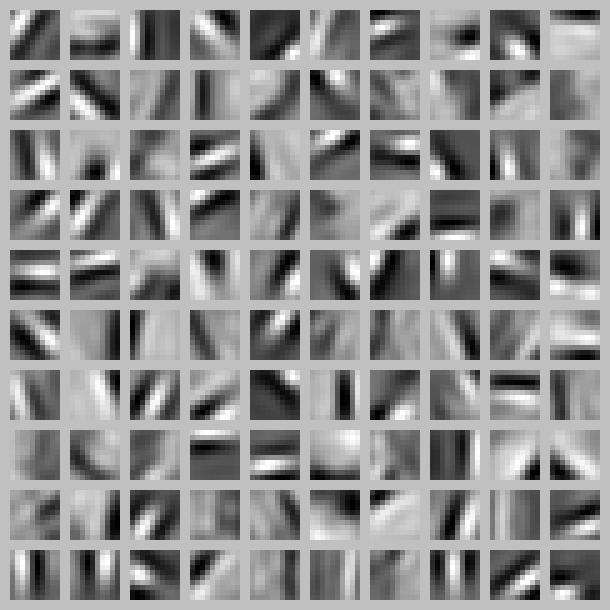
\includegraphics[scale=0.3]{image/autoencoder.png}
\label{fig:autoencoder}
\caption{The features learned from MNIST dataset. Each image correspond to edge at different location and orientation.}
\end{figure}

Supervised feature learning works with labeled image. One technique that successfully implement this idea is Convolutional Neural Network (ConvNet). It is originally proposed by LeCunn et al. \cite{lecunn1999} for handwriting document classification. This method is starting to gain momentum with the success of the seminal work of Krizhevsky et al. \cite{krizhevsky2012cnn} that produce stellar performance, by beating previous state-of-the-art method by large margin, on the ImageNet large scale recognition problem \cite{imagenet}. 

Part of this success can also be attributed to the abundance of labelled training data. ImageNet contains 1.2 million labelled training images from 1000 different categories. Another factor is the advance in Graphical Processing Unit (GPU) which makes training large amount of data feasible. Combining these factors with the learning capacity of a ConvNet makes the result possible.

\begin{figure}[h]
\centering
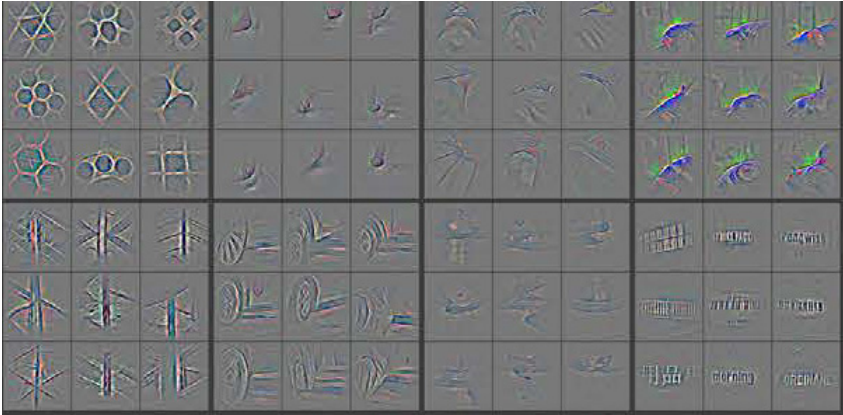
\includegraphics[scale=0.3]{image/cnn.png}
\label{fig:cnn}
\caption{Visualization of features learned from ConvNet.}
\end{figure}
[Visualization of features learned from ConvNet that generalize well to other dataset]

Figure \ref{fig:cnn} shows the example of features learned from a ConvNet, taken from Zeiler and Fergus \cite{zeiler2014} paper. Further research has showed that the feature produced from this network to be highly discriminative, even across different tasks and datasets. Study by Razavian et al. \cite{razavian2014} shows that the features coming from the last second fully-connected of ConvNet trained on ImageNet with simple linear classifier such as Support Vector Machine (SVM) produced top and near state-of-the-art performance in many typical vision tasks such as object classification, fine-grained recognition, and image retrieval. 

The result is pushed even further by finetuning the network with the target dataset. Finetuning works by taking the previously trained network, for example, the AlexNet, and retrain it with target dataset. This works particularly well, rather than training the network from beginning, especially if the target dataset has limited number of training data. This kind of learning, transfer learning, has been reported to produce better result on many occasions \cite{azizpour2014}.

One of the latest example that utilize this power of finetuning is the algorithm Region with CNN (RCNN). RCNN is a object detection algorithm that combines the highly discriminative features with a better search strategy. RCNN employs region proposal algorithm, selective search, that return ~2000 regions that is very likely to contain object. These two makes RCNN to get state-of-the-art result on benchmark dataset and made impressive improvement over previous methods.

This thesis work tries to extends the usability of RCNN. The standard RCNN needs the exact bounding box annotation for each object in the image for finetuning. However, this kind of annotation is more expensive than simply labeling the whole image. Therefore, we tries to bypass this needs and figure out a way to finetune with only whole image label. This kind of learning between the fully supervised and unsupervised is dubbed as weakly supervised learning.

The proposed general setup is as follows. First, we use a region proposal algorithm that can give confidence score that shows how likely a region to contain object. There are several possible candidates such as objectness \cite{obj} and EdgeBoxes. Hosang et al. \cite{hosang2014} provide extensive review of popular algorithm and then outline their strength and flaws. We pick top k regions and then extract them into individual image and and give the label from their source, whole image label.

These regions are then used for finetuning ConvNet that has previously been trained using ImageNet 1.2 million training images in 300,000 more iterations. This finetuned network will then be fed to the standard RCNN pipeline. The performance will be assessed using PASCAL 2007 detection dataset. It will be compared to the non-finetuned network, finetuned network with object bounding box annotation, and network finetuned with whole image.


\chapter{Literature Review}
\section{Convolutional Network (ConvNet)}
Convolutional Neural Network (ConvNet) is a variant of a standard neural network. Here in this section, the development of neural network leading up to ConvNets is briefly described.

\subsection{Artificial Neural Network}
% Single neuron
The first neuron model is proposed by McCulloch and Pitts  In this case, the input vector is multiplied with a weight vector. If this value exceed certain threshold, then this network is firing.

[figure of neuron]

Or in other words $ y = $ where $ a = \sum x_i * w_i $.
\begin{equation}
	\begin{cases}
	1 & \text{if } x \geq \theta \\
	0 & \text{otherwise}
	\end{cases}
\end{equation}

To update the network, there are two alternative. The perceptron rule or Delta rule.

Delta rule, also known as Widrow-Hoff rule, before the output

This kind of architecture act as linear classifier.

% Multi level neural network
This layer can be stacked to become a multi-layer network. Popularized as Multi Layer Perceptron even though it is not using perceptron learning rule. The caveat is then how to update the weight of the network, because we only know the error from the last layer.

The solution is by using threshold-like function, such as sigmoid function, and then performing chain rule to derive the learning update formula. This update formula is known as Backpropogation.

Two popular choice for sigmoid function is $\frac{1-e^{-x}}{1+e^{-x}}$ or $arctan(x)$.
[plot sigmoid function]

This network can be used to approximate all functions, given enough hidden neuron.

\subsection{ConvNet}
A Convolutional Neural Network (ConvNet) is a variant of the multi layer neural network. It is inspired by the visual cortex in retina, where there are small sub-region in the cell that are sensitive, called receptive field.

There are several different paradigms of ConvNet than regular network.
The first is sparse connectivity. A neuron in this case do not need to be connected to all the neurons from the previous layer. For example, a neuron in layer i only need to be connected to limited number of spatially adjacent neuron on layer i-1.
This correlates with the receptive field concept.
[figure sparse]

The second is shared weight. Creating a feature maps. This will ensure that the distinct features will be detected regardless of their position in the image.
It also reduces the number of parameter that needs to be trained.
[figure shared]

Another important concept is max-pooling. Max-pooling partitions the image into non-overlapping rectangular region, and for each region, outputs the maximum value. It has the advantage of reducing the computation cost and also provide some form of translation invariance into the network.


There are other design by choice.
First, Rectified Linear Unit (ReLU) as the activation function. $max(a, 0)$
This vector. However, as ReLU is not differentiable at all points, a conjugate gradients is used and a little modification is used
[plot relu]
Dropout, for regularization to prevent overfit.

Maybe the most famous ConvNet, the AlexNet.
[figure of alexnet]

This network is composed of 5 convolutional layers, followed by 2 fully-connected layers and softmax layer to generate prediction.
This model is trained using GPU for 2 weeks with 1.2 million training data and achieved state-of-the-art performance and fire.

In the past, before ConvNet dominates, a bag of visual word using combined features from HOG, SIFT, and LBP is used.

\section{Region with CNN (RCNN)}
RCNN is the latest object detection algorithm that producing state-of-the-art result on many benchmark dataset such as PASCAL 2007 and ImageNet detection problem.

Object proposal
There is a big shift in how object detection is performed in past. Not so long ago, a densely sampled sliding window is performed to check the location of an object exhaustively in every possible position, scale, and aspect ratio. This can be too time-consuming.

By utilizing multiple cues. Then the time saved can be invested into better and more complicated representation.
Selective Search performs hierarchical grouping from oversegmented region produced from Felzenszwalb and Huttenlocher graph segmentation algorithm. The grouping is done based on multiple criterion. Higher number of proposal is obtained from combining the result from different parameters.
Hosang et al. provide comprehensive evaluation of popular object proposal algorithm.

Domain specific fine-tuning.
Labeled data are scarce. RCNN alleviate this by using supervised pre-training of. In this thesis, we use pre-trained model provided by Caffe.

First, RCNN extract region proposal, around 2,000 proposal for each image using region proposal algorithm such as Selective Search. Then each region is warped to match the size of the ConvNet network. The features from the last fully-connected layer are then extracted. This features is then classified using pre-trained SVM classifier.

[figure rcnn system]

One benefit of RCNN is the decoupling of feature extraction and region detection. This way, we can use possibly a smarter region proposal algorithm, or use different representation using stronger network.

\chapter{Experiment and Result}
\section{Dataset}
The dataset used is PASCAL Visual Object Class 2007. This dataset contains nearly 10000 images of 20 different visual classes.

To validate, first we perform the baseline, as done in the RCNN paper.

We are using Caffe.
Caffe is designed so an experiment parameter can be changed by changing the parameter prototxt file.
There is a pre-trained model which mimic, with different. It is reported 2\% accuracy different.

This is the result.

We then finetune the network with. The strategy is as defined in the paper. Every region with 0.5 is considered as positive samples and.

Because the number of samples can easily reach million of datapoints, negative hard mining is performed.

\bibliographystyle{plain}
\bibliography{ref.bib}

\appendix
\addappheadtotoc
\chapter{RDF}\label{appA}

\begin{figure}[ht]
\begin{center}
And here is a figure
\caption{\small{Several statements describing the same resource.}}\label{RDF_4}
\end{center}
\end{figure}

that we refer to here: \ref{RDF_4}
\end{document}
